\chapter{Revisão bibliográfica}
\label{Cap:RevisaoBibliografica}
\newcommand{\WidthAlgumaCoisa}{6.5 cm}


% Capítulo 2: Revisão Bibliográfica
Este capítulo detalha toda revisão literária aplicada ao projeto,  abordando assim conceitos teóricos, tecnologias e contexto histórico.

\section{Dashboard}

\par O Dashboard, também chamado de painel de controle, é uma ferramenta que auxilia os gestores a terem uma visão mais sistemática das principais informações do negócio. Em outras palavras, é um recurso que visa consolidar os dados de maior relevância em um painel, facilitando o processo de análise e a tomada de decisão.

\par O uso de planilhas e relatórios já são ultrapassados para análises de dados, não sendo suficientes para suprir as necessidades mais urgentes. Conforme a tecnologia foi evoluindo no mundo corporativo, surgiram os dashboards que evitam esforços desnecessários e ter uma visão mais ampla de todo o cenário corporativo para, assim, tomar decisões estratégicas e assertivas.

\par A visualização de dados através de dashboards já é uma realidade em softwares de gestão empresarial, integrando painéis de controle com inteligência artificial e fornecendo informações atualizadas automaticamente. É possível personalizá-los e comparar dados através de filtros, que facilitam análises de indicadores.


\subsection{Uma ferramenta de apoio à decisão}

\par Segundo um estudo feito pela UNINDU (The International Congress on University Industry), 83% das pessoas absorvem melhor as informações através da visão. Isso demonstra a importância do dashboard para tomada de decisões rápidas e melhor análise dos indicadores,melhorando metas e atingindo objetivos.

\par O Business Intelligence (BI), por exemplo, é uma área que exige precisão na coleta e controle das informações para gerar insights em base desta ferramenta. Os dados são agrupados em conjuntos de registros e disponibilizadas por meio de dashboards para mensurar o desempenho atual e futuro da empresa de acordo com o cenário.

\par Além disso, os dashboards monitoram os dados, com o intuito de melhorar todos os processos. Eles permitem que o usuário personalize painéis e filtre informações para a visualização dos resultados, como quantidade, tempo e outras opções.

\subsection{Benefícios do uso para as empresas}

A aplicação dos dashboards na gestão empresarial traz muitos benefícios para a tomada de decisão e a visão estratégica do seu negócio. 

\subsubsection{Auxilia na tomada de decisões}
\par O processo de tomada de decisões fica cada vez mais fácil através dos dashboards, que centralizam informações de fácil visualização e compreensão, possibilitando uma visão ampla do seu negócio. 

\subsubsection{Transparência de informações}
\par Na gestão, é importante que todas as equipes tenham acesso aos indicadores da empresa, mantendo a transparência das informações. As ferramentas de dashboard tem o objetivo de facilitar a comunicação interna entre todos os profissionais.

\subsubsection{Otimização de tempo e recursos}
\par A visualização por dashboards otimiza o tempo para tomarem decisões e evitarem trabalhos manuais e complexos com a organização de dados, passando a priorizar outras atividades mais relevantes.

\subsubsection{Alinhamento estratégico}
\par Com as informações consolidadas em um único painel, a gestão se torna mais ágil e efetiva, possibilitando o alinhamento de estratégias e decisões para o negócio.

\subsection{Antecipação de problemas}

\par Como o dashboard trabalha com atualizações constantes e análises mais específicas, é mais fácil prever problemas e tendências negativas que podem vir a acontecer. Estes problemas ficam mais explícitos com o uso da tecnologia de inteligência artificial que os identifica de maneira mais fácil.

\par Qualquer mudança é detectada com mais simplicidade e o tempo para pensar nas possíveis soluções se torna muito maior. Isso melhora o processo de tomada de decisão e evita possíveis prejuízos. 

\subsection{Experiência de uso}

\par Uma boa interface e uma boa experiência de uso se dá pela arquitetura das informação do dashboard. É fundamental que seja organizado, coerente e intuitivo. O objetivo é tornar o mais fácil possível encontrar o que se procura. Através de menus, cores e  símbolos é possível saber quais são as opções e deixar claro as consequências que cada ação irá gerar. Dessa forma, a experiência do usuário ao usar o dashboard será rápida e efetiva, atendendo suas expectativas.

\section{Inteligência Artificial, Machine Learning e Deep Learning}

\par A Inteligência Artificial ganhou destaque mundialmente nos últimos anos como um importante e rentável campo da computação. A situação não é diferente no Brasil. Uma pesquisa realizada pela Microsoft, em 2019, revela que em um cenário de máxima utilização de inteligência artificial no Brasil, a taxa composta anual de crescimento (CAGR) do Produto Interno Bruto (PIB) pode aumentar para 7,1\% ao ano, até 2030.

\par Andreas Kaplan e Michael Haenlein definem a inteligência artificial como “uma capacidade do sistema para interpretar corretamente dados externos, aprender a partir desses dados e utilizar essas aprendizagens para atingir objetivos e tarefas específicos através de adaptação flexível”.

\par Um dos campos da Inteligência Artificial é o Machine Learning (Aprendizado de Máquina), que por sua vez pode ser definido como a capacidade de uma máquina, baseando-se em algoritmos e nos dados que estão sendo analisados possa tomar decisões capazes de resolver problemas ou prever comportamentos.

\par Existem duas maneiras de uma máquina aprender, criando duas categorias do Machine Learning, sendo elas aprendizagem supervisionada e aprendizagem não supervisionada. Na aprendizagem supervisionada, o cientista de dados é o responsável por monitorar o algoritmo, que irá aprender baseado em conhecimentos e experiências prévias. Resumidamente, que nessa categoria, sabe-se a saída que o algoritmo deve chegar tendo como base uma entrada. Como exemplo, pode-se citar a classificação de imagens e detecção de objetos.

\par Por outro lado, na aprendizagem não supervisionada, não existe um resultado específico esperado e o algoritmo irá aprender com base nos próprios dados que estão sendo processados. Em geral, necessita-se de um maior volume dados. Como exemplo, pode-se citar o processamento de linguagem natural para criação de legendas automáticas.

\par Por fim, dentre outras abordagens do Machine Learning, encontra-se o Deep Learning (Aprendizado Profundo), objeto de estudo deste trabalho, que é capaz de resolver problemas do mundo real por meio de redes neurais artificiais certas vezes com mais precisão e velocidade do que humanos. 

\begin{figure}[H]
    \centering
    \caption{Inteligência artificial, aprendizado de máquina e aprendizado profundo}
    
\includegraphics[width=1.0\linewidth]{Imagens/deep.png}
    \caption*{Fonte: Arquivo dos autores (2020)}
    \label{autoai-results}
\end{figure}

\section{Deep Learning e Redes Neurais}

\subsection{História}
\par O início da história do deep learning data de 1943, quando o matemático Walter Pitts e o neurofisiologista Warren McCulloch, baseando-se em pesquisas do cérebro humano, modelaram o primeiro modelo computacional para uma rede neural, baseando-se em neurônios simples, criados a partir de circuitos elétricos. Walter e Warren utilizaram uma combinação de matemática e algoritmos, denominada de lógica de limiar (threshold logic), que é utilizada até os dias atuais como base das redes neurais.

\par Em 1960, Henry J. Kelley desenvolveu o conceito básico de um modelo de retropropagação (backpropagation), que também é utilizado até os dias atuais para o recálculo dos pesos das redes neurais no processo de aprendizagem. Apesar das descobertas e estudos nas décadas entre 40 a 80, devido à limitação computacional existente na época, o aprimoramento das redes neurais foi severamente impactado até 1981 e o assunto foi subestimado e criticado, além de ter sofrido grande redução no financiamento de pesquisas relacionadas à área.

\par Entretanto, em 1982, John Hopfield apresentou uma abordagem prática para redes neurais, demonstrando como elas poderiam atuar em problemas reais, o que fez com que o assunto voltasse a ter sua devida atenção. Em 1987 ocorreu a primeira Conferência Internacional sobre Redes Neurais do Institute of Electrical and Electronic Engineer’s (IEEE). Ao mesmo tempo que o assunto vinha novamente ganhando destaque, o poder computacional da época ainda não conseguia acompanhar o desenvolvimento dos estudos, impossibilitando a criação de grandes aplicações com deep learning, o que gerou frustração e novamente uma redução de investimentos na área.

\par Ainda assim, algumas pessoas continuaram estudando o assunto e em 1995, Dana Cortes e Vladimir Vapnik desenvolveram a máquina de vetores de suporte, um sistema capaz de reconhecer padrões com aprendizado supervisionado. Nos anos seguintes, a partir de 1999, os computadores começaram a ganhar poder de processamento, viabilizando a implementação de redes neurais mais eficientes, que começaram a competir com as máquinas de vetores de suporte. Apesar de possuírem um maior tempo de processamento, em geral, as redes neurais se mostraram mais assertivas utilizando os mesmos dados e voltaram a ganhar visibilidade no mercado.

\par A partir de então diversos estudos e pesquisas realizados na área e à medida que os computadores foram evoluindo, as aplicações envolvendo redes neurais também o fizeram. Nos anos subsequentes, o algoritmo de aprendizagem profunda do Google foi capaz de identificar gatos em 2012 e em 2014 o Facebook implementou a DeepFace, tecnologia capaz de marcar automaticamente os rostos dos usuários da rede social em fotografias. Dois anos depois, o algoritmo do Google AlphaGo mapeou o jogo de tabuleiro Go e ganhou de Lee Sedol em um torneio em Seul, que à época tinha sido campeão mundial de Go 18 vezes.

\par Com isso, o campo da inteligência artificial e do deep learning em especial vem avançando em pesquisas até os dias atuais, além de novamente ter ganhado visibilidade e estar inserido em diversas aplicações corporativas que requerem uma análise de dados mais profunda, com reconhecimento de padrões, previsões ou classificações, por exemplo.

\subsection{Funcionamento das Redes Neurais}

\par O funcionamento das redes neurais atuais pode ser explicado tendo como base o perceptron elementar, o modelo mais simples e didático de rede neural de camada única.

\begin{figure}[H]
    \centering
    \caption{Perceptron Elementar}
    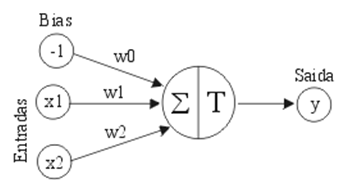
\includegraphics[width=0.6\linewidth]{Imagens/perceptron.png}
    \caption*{Fonte: UFSC, s.d. (\url{https://www.gsigma.ufsc.br/~popov/aulas/rna/neuronio_implementacao/})}
    \label{perceptron}
\end{figure}

\par No modelo apresentado (Figura \ref{perceptron}), constituído por apenas um único neurônio artificial, duas entradas, uma unidade de bias e uma saída, cada entrada possui pesos w0, w1 e w2 associados a elas, assim como a unidade de bias, que também funciona como uma entrada, mas possui seu valor fixado normalmente em 1 ou -1, com a finalidade de aumentar o grau de liberdade do ajuste dos pesos. Por padrão, em bibliotecas que possibilitam a implementação de redes neurais, a unidade de bias já é definida automaticamente.

\par Assim sendo, o algoritmo \cite{UNIUBE2020} que simula o neurônio irá multiplicar cada entrada por seu respectivo peso para todas as entradas e realizar a somatória de todos esses resultados. Após a obtenção do valor da somatória, ele deve ser submetido a uma função de ativação ou transferência T, gerando a saída y. Dentre outras funções de transferência, pode-se citar a função sigmoide, tangente hiperbólica, unidade linear retificada (ReLU) e unidade linear exponencial (ELU).

\par Durante os estudos e desenvolvimento de algoritmos para redes neurais, ficou claro que para problemas mais complexos, seria necessário expandir a quantidade de neurônios e de camadas, tornando a saída de um neurônio, a entrada para o próximo. A quantidade de neurônios e de camadas deve ser estudada e testada individualmente para cada problema que se pretende solucionar, variando caso a caso.

\begin{figure}[H]
    \centering
    \caption{Rede Neural Multicamada}
    
\includegraphics[width=1.0\linewidth]{Imagens/rede-neural.png}
    \caption*{Fonte: Arquivo dos autores (2020)}
    \label{redeneural}
\end{figure}

\par As redes neurais artificiais multicamadas são divididas basicamente em três principais partes: entradas, camadas ocultas e saída, podendo ser uma ou várias dependo do tipo de problema. Nesse tipo de rede, uma série de neurônios são interligados como mostrado e quando uma saída é obtida, ela é comparada com uma saída considerada correta, gerando um valor de erro. Com base nesse erro, os pesos são então recalculados utilizando o conceito de gradiente para a minimização do erro, até que seu valor seja considerado satisfatório. Essa etapa em que os pesos são recalculados e a rede neural está sofrendo alterações é denominada de treinamento.

\par Após essa fase, a rede deve ser testada com dados diferentes dos que foram usados durante o treinamento para garantir sua assertividade. Essa etapa recebe o nome de teste. Caso comprovada sua eficiência e as taxas de erro permanecerem baixas, a rede neural está apta para ser utilizada com dados novos obtidos de um contexto real.



\section{Assunto 3}

XXXXXX
\\\\
XXXXXX

\subsection{SubAssunto 3}

XXXXXX
\\\\
XXXXXX

\section{Análise de Dados}

\par Apesar de estar cada vez mais em destaque nestes últimos anos, podemos traçar o uso de estatística para tomada de decisão desde do Egito Antigo, de acordo com um artigo publicado por Keith D. Foote os egípcios já usavam cálculos estatísticos para construir as pirâmides. Já na década de 1880, o governo americano levou pelo menos 7 anos para completar o censo da população, processo que foi reduzido para um ano e meio na década seguinte por causa do desenvolvimento de uma máquina de tabulação, por Herman Hollerith, que processava os dados de forma sistêmica em cartões perfurados.

\subsection{Primeira fase da análise de dados}

\par Trazendo para os dias atuais, a Universidade de Villanova separa a análise de dados em três estágios. O primeiro deles seria o início do que chamamos de Business Intelligence, que surgiu por volta de 1950 como uma forma de processar pequenas quantidades de informações estruturadas. Esse estágio, que podemos chamar de Analytics 1.0, durou até cerca de 2009, quando foi consolidado o termo "big-data".

\par O fim do primeiro estágio se deu pelo aumento exponencial de dados sendo produzidos diariamente, podendo vir de qualquer lugar e forma, desde de informações simples e estruturadas, como quais produtos alguém comprou em um determinado site, ou coisas mais complexas, como quais sites fizeram essa pessoa chegar até uma determinada página e qual a posição geográfica dessa pessoa quando acessou a página. Se convencionou a chamar esses dados em grande quantidade e pouco estruturados de "big-data".

\subsection{Segunda fase da análise de dados}

\par Pela dificuldade de armazenar e processar essa massiva quantidade de dados, se fez necessário o desenvolvimento de novos métodos e ferramentas para o processamento deles, o que deu início ao Analytics 2.0, que trouxe alternativas como Hadoop, que pode processar essas grandes massas de dados, e o NoSQL, que permite armazenar toda a informação de forma mais eficiente que os bancos de dados relacionais faziam até então. Além disso, cada vez mais se fez necessário um conhecimento tecnológico para fazer essas análises, quando até então bastava o conhecimento de métodos estatísticos.

\subsection{Terceira fase da análise de dados}

\par Hoje em dia, muitos especialistas dizem que chegamos a um terceiro estágio, o Analytics 3.0, onde esses dados que são produzidos a qualquer momento podem ser usados como moeda de troca entre consumidor e fornecedor. Essa moeda pode ser analisada imediatamente pelo fornecedor, que passa a entregar uma experiência personalizada para quem está consumindo o seu produto.

\subsection{Análise de dados no dia a dia}

\par Com a disponibilidade de dados que temos, as empresas estão se dedicando cada vez mais em coletar e auxiliar as suas decisões nas análises feitas com eles. O Diretor de Estratégia e Marketing de Precisão da Coca-Cola, Justin De Graaf, afirmou em entrevista para ADMA, Association for Data-Driven Marketing \& Advertising, que cada vez mais a empresa usa informações coletadas diretamente dos consumidores, como por meio de telefone, redes sociais ou e-mail, para criar desde campanhas publicitárias até novos produtos. Outra marca consolidada usando análise de dados para a tomada de decisão é a rede de hotéis Marriott, que, de acordo com o seu chief development officer, Eric Jacobs, tem usado esse tipo de informação para decidir como identificar, atrair e manter os seus cliente mais lucrativos. Para isso eles coletam desde dados como padrão social dos clientes até se eles consomem mais jeans Levi's ou Gap.

\par Apesar disso, alguns resultados dessas análises podem ter um efeito contrário do que era pretendido no início. Caso a análise não seja feita com atenção, verificando sempre quem está sendo atingido, ela pode levar a alguns atritos e desgastar a imagem de quem usa essas informações.

\par Em 2012, o New York Time publicou uma história de como um pai descobriu a gravidez da filha através de uma promoção oferecida pela rede varejista Target, nos Estados Unidos. Andrew Pole, um estatístico da rede, foi designado para desenvolver um "preditor de gravidez", no fim do estudo ele conseguiu chegar a uma lista de 25 produtos, que geram uma probabilidade da cliente estar grávida de acordo com o seu preditor. Esses produtos contêm itens como manteiga de cacau, bolsas grandes o suficiente para caber pacotes de fraldas, e suplementos como magnésio e zinco.

\par A Target vinculava essa informação a um identificador do cliente, e então ofereceria um desconto na próxima visita que essa mesma pessoa fizesse a loja. Um ano após a aplicação deste preditor, o pai de uma adolescente foi a uma das lojas reclamar que sua filha tinha recebido um desconto relacionado a esse programa específico para grávidas, com isso, o gerente da loja se desculpou pelo erro e alguns dias depois ligou para se desculpar novamente. Entretanto, para a surpresa do gerente, durante essa ligação o cliente disse que a filha não tinha contado para ele que estava grávida, e que a Target soube antes dele do acontecido. Após esse caso, o departamento de marketing decidiu desacelerar o programa de análises de dados, e passar mais tempo avaliando qual impacto cada iniciativa pode ter.

\section{Tecnologia de Monitoramento de Ônibus}

\par De acordo com a informação exposta em uma publicação feita em 2017 pela Escola de Negócios da Universidade de Indiana, era previsto um crescimento anual de mais de 23\% no mercado de Big Data durante o período de 2014 a 2019, com um custo de \$48,6 bilhões no último ano. Isso inclui um crescimento de 30\% entre 2014 e 2015 de aparelhos conectados e dispositivos de IoT. Estes aparelhos geram uma quantidade enorme de dados valiosos para quem tiver interesse de processá-los.

\par Esse cenário hoje não é diferente para o setor de transporte público, com a prefeitura de Santo André capturando dados em tempo real da sua frota de ônibus, informações como bilhetagem, velocidade e paradas dos veículos, porém não utilizando a informação para a tomada de decisão.

\par Um exemplo de uso prático desses dados foi publicado em um artigo da IEE, para a Conferência Internacional da Logística e Transporte Avançado. Em uma colaboração entre a IBM e o Conselho da Cidade de Dublin foi realizado um projeto de cidade inteligente entre 2010 e 2013. A IBM passou a processar os dados gerados pela frota de ônibus, além de outras fontes, com intenção de reduzir o trânsito na cidade sem precisar alterar a sua estrutura atual, que conta com vários pontos históricos.

\par O inicio do processo se dava com informações coletadas do ônibus, como dados de GPS, velocidade, paradas e bilhetagem, e depois eram adicionadas novas informações vindas de sistemas de semáforos, CCTV, sistemas meteorológicos, entre outros. Todos esses dados então eram processados em um servidor da IBM e disponibilizados em mapa em tempo real do transporte público de Dublin.

\par Com toda essa informação processada, a cidade teve uma maior capacidade de monitorar o seu sistema de transporte público, diminuindo o tempo para uma tomada de decisão.

\par Outro exemplo de aplicação de tecnologia no monitoramento de transporte coletivo é do USapiens, um sistema desenvolvido por um time de pesquisa da IBM do Brasil. Essa equipe usou dados de transporte coletivo da cidade do Rio de Janeiro para desenvolver um sistema que processa os dados recebidos pelo GPS dos ônibus e depois disso analisa-se por diversos modelos esses dados.

\par Para isso eles integraram os dados obtidos pelo GPS com informações disponíveis de GTFS, sigla para General Transit Feed Specification, que contém dados mais gerais das rotas de ônibus, como paradas e horários esperados. Feita essa integração, os dados são limpos para prevenir problemas como latitude/longitude imprecisas ou dados com intervalo de tempo muito grande. Com os dados prontos, é feita uma comparação com a rota do GTFS, se descobre a direção do veículo e com isso tem seu trajeto normalizado em uma escala de distância e tempo acumulativas.

\par Com a informação normalizada, o sistema pode ajudar a responder três perguntas principais. Através de uma análise descritiva histórica podemos responder "O que aconteceu e porque?", analisando os dados em tempo real se responde "O que está acontecendo e porque?" e uma análise preditiva responde "O que vai acontecer e porquê?".

\par Os pesquisadores da IBM depois aplicaram esse sistema a 5 casos de estudo. O primeiro foi uma Análise de Uniformidade dos Ônibus, para evitar um agrupamento de veículos na linha, o segundo caso foi uma verificação na rotas dos ônibus, para avaliar a aderência do veículo a sua rota pré-definida, o terceiro uma análise de fluxo no trânsito, o quarto a variância do tempo de viagem do veículo, que permite avaliar a consistência da rota analisada, e para o quinto ele usaram a análise preditiva para prever o tempo de chegada do ônibus.


